\subsubsection{pn-Junction Diode}
The following circuit is used to analyze the transient responses or switching behaviors of pn-junction diodes, Schottky diodes, and switching diodes:
\FloatBarrier
\begin{figure}[h!]
	\centering
	\caption{Circuit Schematic for Diode Transient Response Analysis}
	\label{fig:dtr}
\begin{circuitikz} \draw
	( 0 , 4 ) to [ sqV , v<=$20Vpp$ ] ( 0 , 0 )
	( 0 , 4 ) to [ empty diode ] ( 4 , 4 )
	( 4 , 4 ) to [ R = 300 <\ohm> ] ( 4 , 0 ) -- ( 0 , 0 ) ;
\end{circuitikz}
\end{figure}
\FloatBarrier

The empty diode represents the different types of diodes analyzed and a square source with positive edge at $10V$ and negative edge at $-10V$ is used ($20Vpp$) with a frequency of $10 kHz$. The positive and negative edges of the square source applies a forward and reverse bias respectively on the tested diodes. Because of the sharp transition from the positive to negative edge of the source, switching behavior is to be observed in the diode circuit.

When forward bias is applied to a pn-junction diode, an electric field is generated across the diode from the p-region to the n-region. This causes excess holes from the p-region to migrate across the depletion region to the n-region and excess electrons from the n-region to migrate to the p-region. The migrated charge carriers are the excess minority charge carriers of the quasi-neutral regions that they migrated to and are effectively "stored" in the new regions that they reside in. The current through the diode after an adequately long duration of time reaches a constant current, $I_{F}$, at steady state.

When the square source wave undergoes the sharp transition from its positive to negative edge, a reverse bias is abruptly applied to the pn-junction diode and the electric field across the pn-junction diode is immediately reversed. The reversal in polarity of the electric field causes the excess minority carriers to flow out of their respective quasi-neutral regions and recombine with donor and acceptor ions on the other side. This movement of carriers causes a reverse current, $I_{R}$, that is much greater in magnitude than the reverse saturation current, $I_{S}$ (ideally, $I_{S}$ is approximately $0.1I_{R}$). The withdrawal of the stored excess minority carriers across the depletion region causes the reverse current to be close to constant for a duration called the storage time, $t_{s}$. After that period of time, the reverse current then decays to the reverse saturation current.

The storage time, $t_{s}$ is ideally represented in the following equation:
\begin{equation}
\label{eq:diode_t_s}
erf(\sqrt{\frac{t_{s}}{\tau_{p}}}) = \frac{1}{1+\frac{I_{R}}{I_{F}}}
\end{equation}
where $\tau_{p}$ is minority carrier lifetime and $erf(\xi)$ is the error function defined to be:
\begin{equation}
\label{eq:erf}
erf(\xi) = \frac{2}{\sqrt{\pi}}\int_{0}^{\xi}e^{-x^{2}}dx
\end{equation}

Effectively, because of the interactions of excess charge carriers within the pn-junction diode, a delay is to be observed in the rectification of the reverse signal and the current waveform of the pn-junction diode should have the following shape:
\FloatBarrier
\begin{figure}[h!]
	\centering
	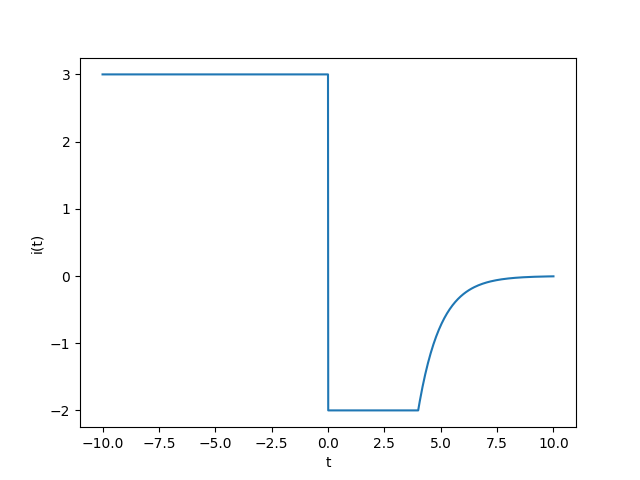
\includegraphics[scale=0.75]{./images/diode_current.PNG}
	\caption{pn-Junction Diode Expected Current Waveform}
	\label{fig:diode_current}
\end{figure}
\FloatBarrier
Also, the voltage waveform of the diode should also have an observable delay in switching polarity and the waveform should look like the following:
\FloatBarrier
\begin{figure}[h!]
	\centering
	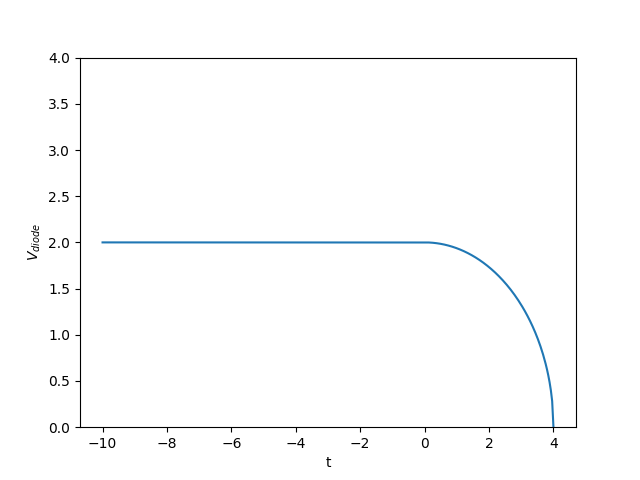
\includegraphics[scale=0.75]{./images/diode_voltage.PNG}
	\caption{pn-Junction Diode Expected Current Waveform}
	\label{fig:diode_voltage}
\end{figure}
\FloatBarrier
*Note that for both Figures (\ref{fig:diode_current}) and (\ref{fig:diode_voltage}), the source voltage switches at $t=0$.

In the observation of the pn-junction diode, the following waveform is observed for the voltage across the $300\Omega$ resistor where the top wave is the voltage across the resistor and the bottom wave is the source voltage:
\FloatBarrier
\begin{figure}[h!]
	\centering
	\includegraphics[scale=0.25]{./images/pn_junction_diode_transient_response.jpg}
	\caption{pn-Junction Diode Observed Voltage Across Resistor}
	\label{fig:pn_diode_v_r}
\end{figure}
\FloatBarrier
The following waveform is then observed for the voltage across the pn-junction diode:
\FloatBarrier
\begin{figure}[h!]
	\centering
	\includegraphics[scale=0.25]{./images/pn_junction_diode_v_diode.jpg}
	\caption{pn-Junction Diode Observed Voltage Across Diode}
	\label{fig:pn_diode_v_d}
\end{figure}
\FloatBarrier
The forward and reverse voltages of the pn-junction diode are then measured to be the following:
\begin{equation}
\label{eq:pn_measured_vfr}
V_{F}=8.375V,V_{R}=-9.8125V
\end{equation}
The current through the diode and the voltage across the resistor have a simple Ohmic relationship, so the forward and reverse currents can be found by doing the calculation below:
\begin{equation}
\label{eq:ifr_vs_vfr}
I_{F/R}=\frac{V_{F/R}}{R_L}=\frac{V_{F/R}}{300\Omega}
\end{equation}
The following results for forward and reverse currents are then calculated:
\begin{equation}
\label{eq:pn_measured_ifr}
I_{F}=27.91mA,I_{R}=-32.71mA
\end{equation}

By employing KCL, the following equation can be utilized to find the theoretical value for $I_F$:
\begin{equation}
\label{eq:if_theory}
I_F = \frac{V_P-V_{on}}{R_L}
\end{equation}
and this equation for the theoretical value of $I_R$
\begin{equation}
\label{eq:ir_theory}
I_F = \frac{V_N+V_{on}}{R_L}
\end{equation}
By substituting the values $V_P = 10V$, $V_N = -10V$, and $V_{on} = 0.7V$, the following theoretical values are calculated:
\begin{equation}
\label{eq:pn_theoretical_ifr}
I_{F}=31mA,I_{R}=-31mA
\end{equation}
The percent errors for $I_F$ and $I_R$ respectively are $-10.0\%$ and $-5.5\%$.
\FloatBarrier
\begin{table}[h!]
	\centering
	\caption{Measured vs. Theoretical Forward and Reverse Currents for pn-Junction Diode}
	\label{tab:pn_ifr}
	\csvautotabular{./tables/pn_ifr.csv}
\end{table}
\FloatBarrier

Zooming in to the region in the which the delay occurs allows for the storage time to be more clearly observed and measured:
\FloatBarrier
\begin{figure}[h!]
	\centering
	\includegraphics[scale=0.25]{./images/pn_junction_storage_time_v_resistor.jpg}
	\caption{pn-Junction Diode Observed Storage Time}
	\label{fig:pn_diode_t_s}
\end{figure}
\FloatBarrier
The storage time of the pn-junction diode measured from the oscilloscope is the following:
\begin{equation}
\label{eq:pn_measured_t_s}
t_{s}=2.97\mu s
\end{equation}
After measuring the storage time of three other diodes, the following values for storage times are found:
\FloatBarrier
\begin{table}[h!]
	\centering
	\caption{Measured Storage Times of Various pn-Junction Diodes}
	\label{tab:pn_ts}
	\csvautotabular{./tables/pn_ts.csv}
\end{table}
\FloatBarrier
By observation, the first storage time measurement seems to be an outlier.

\subsubsection{Schottky Diode}
For the Schottky diode, the following waveform for voltage across the resistor is observed (top waveform is source voltage and bottom waveform is the voltage across the resistor):
\FloatBarrier
\begin{figure}[h!]
	\centering
	\includegraphics[scale=0.25]{./images/schottky_diode_input_output_waveforms.jpg}
	\caption{Schottky Diode Observed Voltage Across Resistor}
	\label{fig:schottky_vr}
\end{figure}
\FloatBarrier
The following would then be the observed waveform for voltage across the diode:
\FloatBarrier
\begin{figure}[h!]
	\centering
	\includegraphics[scale=0.25]{./images/schottky_diode_v_diode.jpg}
	\caption{Schottky Diode Observed Voltage Across Diode}
	\label{fig:schottky_vd}
\end{figure}
\FloatBarrier
In both oscilloscope plots (Figures (\ref{fig:schottky_vr}) and (\ref{fig:schottky_vd})), there is no observable delay in the rectification of the source signal for the Schottky diode. This is expected behavior due to the physical features of the Schottky diode. The Schottky diode differs fundamentally from a pn-junction diode in that it utilizes metal-semiconductor junction where the semiconductor is n-type(M-S junction). A depletion region created by the M-S junction is negligible compared to that of a pn-junction (\ref{ref:schottky}). Also, while pn-junction diodes rely on both electrons and holes to carry electric current, Schottky diodes only utilize electrons (\ref{ref:schottky}). Because of this physical property, there are no excess minority carriers that accumulate at quasi-neutral regions, thus no storage time should be observed and switching time is near instantaneous.